
%%% Local Variables: 
%%% mode: latex
%%% TeX-master: t
%%% End: 

\chapter{资源管理可编程体系结构PARD}
\label{chap:pardarch}

Why we need PARD? => single/batch-program change to multi-thread program to multi-tent/cloud
但体系结构几乎没有变化,不能区分不同应用,造成\ref{chap02}中的一些问题。

随着核数增多,单个应用无法用满所有的核,出现了虚拟化技术,其本质是在虚拟地址空间之外增加一层地址空间

本章介绍PARD体系结构与其基本特性,对比PARD与SDN结构,PARD系统使用实例,如何在现有系统中构造出PARD。

% Need of a PARD's labeled address space
\section{标签化地址空间}

%软件层标签化(cgroup/VM),逻辑域,
%标签化用途
%如何实现

多个虚拟地址空间对应一个物理地址空间。
EPT增加了一级地址映射,实现内存划分;I/O MMU技术让硬件设备能够识别EPT增加的一级地址空间。
PCI-E的SR-IOV技术让设备

什么是资源管理可编程体系结构,关键点:
 * Tag机制,实现Labeled Address Space / Performance Space
 * 可编程机制,

%\subsubsection{Key Concept of PARD}
%Key1: Labeled Address Space:机器可划分,细粒度使用
%Key2: 将SDN引入体系结构:中心化管理,可编程


\section{PARD体系结构设计}

%\begin{description}
% \item[First] \hfill \\
% The first item
% \item[Second] \hfill \\
% The second item
% \item[Third] \hfill \\
% The third etc \ldots
%\end{description}

\begin{figure}[htb]
  \centering
  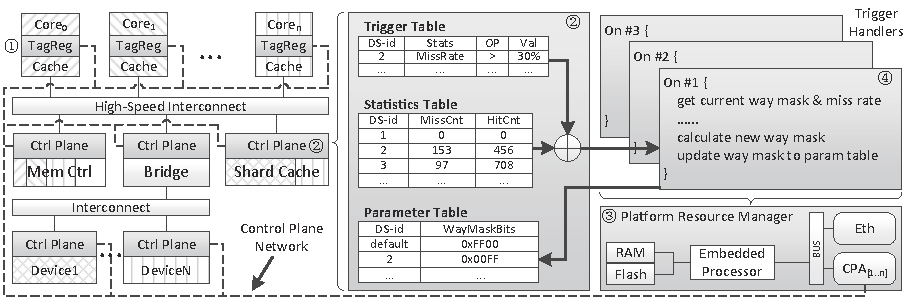
\includegraphics{arch/pard-arch-detail.pdf}
  \caption{PARD体系结构}
  \label{fig:pard-example}
\end{figure}

本研究的目的是在体系结构层次解决数据中心所面临的资源利用率与服务质量相冲突的问题,
论文的主要工作围绕下述三个阶段开展:

\begin{itemize}
 \item 本研究在Xeon E5-v3平台上验证Cache容量划分功能对应用性能隔离带来的作用,
       并提出一种基于反馈模型的缓存自适应分配方法。
 \item 在体系结构内引入标签,实现应用区分,并在各个共享资源对其进行区分处理
 \item 提出一种资源管理可编程体系结构,实现可编程的硬件共享资源的细粒度管理
\end{itemize}

基于PARD的架构,可以很容易实现不同粒度的性能隔离,如虚拟机、进程、线程或基于API的代码/数据段级。
为简化实现与验证,本文在后续章节中使用虚拟机级性能隔离,
在第\ref{chap:future}章中我们将讨论要实现其它级别性能隔离所需要的修改。


\section{PARD示例:用户视图}

本节将以一种虚拟化场景介绍如何利用PARD实现多应用共享硬件,并保证关键应用的服务质量。
本节所述的场景如图\ref{fig:pard-cloud}所示,其中涉及两种角色:
(1)用户,需要使用PARD服务器部署应用,而应用分为延迟敏感型应用与批处理型应用两类;
(1)管理员,管理硬件资源,为用户分配虚拟机以运行应用,同时监控应用性能并对系统进行调整。
在真实的环境中,用户与管理员并不会直接操作服务器本身,而是通过如mesos、OpenStack等集群管理系统使用服务器资源。
这里为了简化描述,将集群管理系统这一层移除,让用户与管理员直接操作服务器。

关键功能+使用方法+流程示意

\begin{figure}[htb]
  \centering
  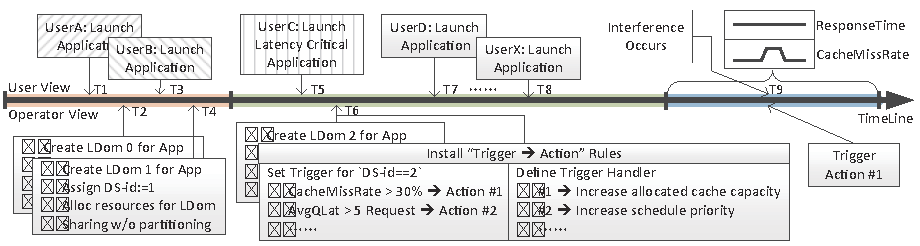
\includegraphics{arch/pard-example.pdf}
  \caption{PARD示例}
  \label{fig:pard-example}
\end{figure}

\subsection{虚拟机创建与关闭}

\subsection{性能监控与反馈}

\subsection{资源调整}

\section{体系结构的可行性}

在X86或ARM上实现该架构

%如何在一个ARM中实现PARD功能

如上节所述,PARD并不是一个完全全新的体系结构,而是对现有体系结构的扩展。
为了说明如何将PARD扩展到一个现有的体系结构中,本节首先构建了一台虚拟计算机,
我们将其命名为XXXX,如图\ref{fig:XXX-computer}所示。
XXX包含两路4核的处理器,每个处理器核拥有独立的一级缓存L1-I和L1-D,
每个Socket的四个处理器核共享一个16路2MB的二级缓存;
两个Socket拥有自己的内存控制器,同时使用MESI目录协议实现NUMA内存访问;
XXX的I/O子系统包含SATA控制器和两个以太网卡,通过IOH芯片与两个处理器相连。
XXX的结构可以很好的匹配到目前流行体系结构中(如X86或ARM)。

\subsection{Computer as a Network => PARD}

\subsection{像SDN一样集中式的管理计算机}

\section{PARD与SDN}

在第\ref{chap:intro}章中我们提出
同时,计算机内部也可以被看做一个网络,如图\ref{fig:computer-as-a-network}所示,
CPU核、共享缓存、内存控制器、I/O设备等可以被看做是网络节点;除了处理请求以外,
这些“网络节点”与网络中的路由器/交换机具有相似的请求转发功能;
而它们之间也通过包进行通信,如:片内通信使用NoC包,片间通信的QPI/HT包,
以及I/O部分使用的PCI-E包。
将网络领域的区分化服务和软件定义网络的思想应用到计算机内部的网络,
用以解决数据中心当前面临的资源利用率与应用服务质量矛盾,是本文的主要研究思路与动机。

与在网络中部署SDN相比,在计算机体系结构“网络”中部署SDN会面临以下三个挑战:

首先,在整个网络栈中EndPoint是唯一的请求来源,因此SDN可以很容易的将标签机制实现在网络栈中;
与之相对的,在计算机体系结构中存在大量的硬件部件都能够发送请求,而这些请求类型又不尽相同,
因此在这样的环境下如何为请求打上标签是一个很大的挑战。

其次,在网络中所有的交换机都执行相同的存储/转发(store-and-forward)操作,但在计算机内部
不同的部件都有不同的功能,而不只是简单的存储/转发,如何为这些不同类型的部件(如末级缓存控制器、
内存控制器、I/O设备等)设计统一的控制面结构是另一个挑战。

最后,在网络交换机中已经包含了一个firmware固件用于访问和配置交换机的控制面,但计算机中却缺少
这样的firmware。现有的IPMI只被用来做有限的监控与管理功能,如对温度、风扇转速和电源控制。
因此,需要在计算机内部提供一种这样的部件实现与其它众多的控制面的通信与管理,并提供一个灵活的
编程接口对这些控制面进行操作。


\begin{figure}[tbh]
  \centering
  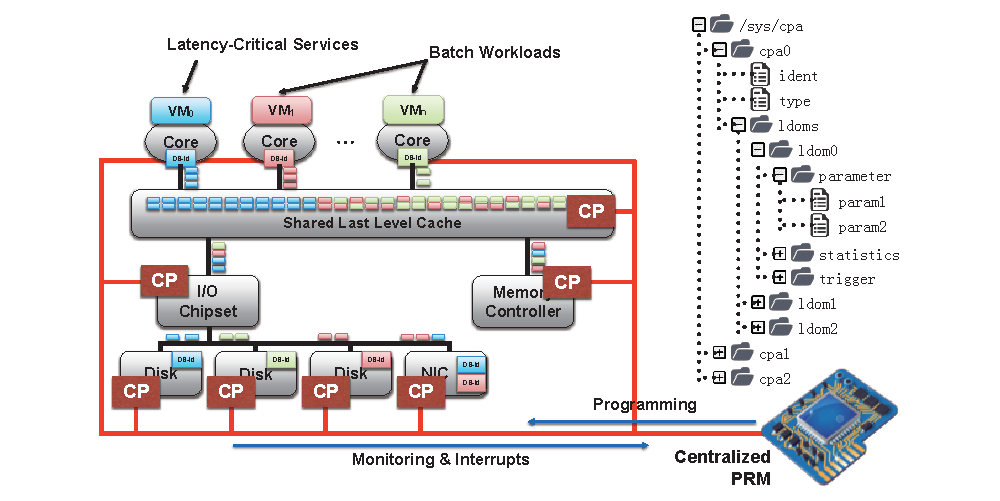
\includegraphics{arch/pard-arch-outline.pdf}
  \caption[PARD体系结构概况]{PARD体系结构概况}
  \label{fig:pard-arch-outline}
\end{figure}

\begin{figure}[tbh]
  \centering
  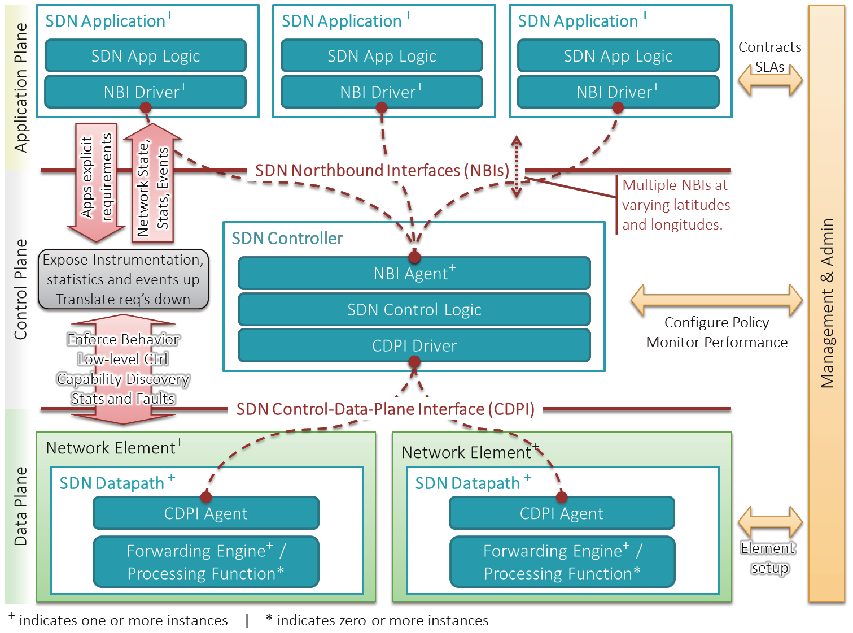
\includegraphics{arch/sdn-arch.pdf}
  \caption{软件定义网络SDN架构}
  \label{fig:pard-arch-outline}
\end{figure}

\section{小结}
